\documentclass[border=6pt,tikz]{standalone}
\usepackage{tikz}
\usepackage{amsmath,amssymb}
\usetikzlibrary{arrows.meta,positioning,fit,backgrounds,calc,shapes.geometric,decorations.pathreplacing,patterns}
\definecolor{ink}{HTML}{1B2430}
\definecolor{muted}{HTML}{6B7785}
\definecolor{accent}{HTML}{2F6FB5}
\definecolor{accent2}{HTML}{C1611F}
\definecolor{good}{HTML}{2E7D5B}
\definecolor{soft}{HTML}{EDF2F7}
\definecolor{soft2}{HTML}{FBEDE2}
\definecolor{soft3}{HTML}{E6F0E9}
\tikzset{
  box/.style={draw=ink,line width=.7pt,rounded corners=2pt,fill=soft,inner sep=4pt,align=center,font=\sffamily\small},
  boxa/.style={box,fill=soft2},
  boxb/.style={box,fill=soft3},
  plain/.style={align=center,font=\sffamily\small,text=ink},
  tiny/.style={align=center,font=\sffamily\scriptsize,text=muted},
  ar/.style={-{Stealth[length=2.4mm]},draw=ink,line width=.7pt},
  arm/.style={-{Stealth[length=2.4mm]},draw=muted,line width=.6pt,dashed},
  nd/.style={circle,draw=ink,line width=.7pt,fill=white,minimum size=7mm,inner sep=0pt,font=\sffamily\scriptsize},
  ndf/.style={nd,fill=soft},
  ndt/.style={nd,fill=soft2},
}

\begin{document}
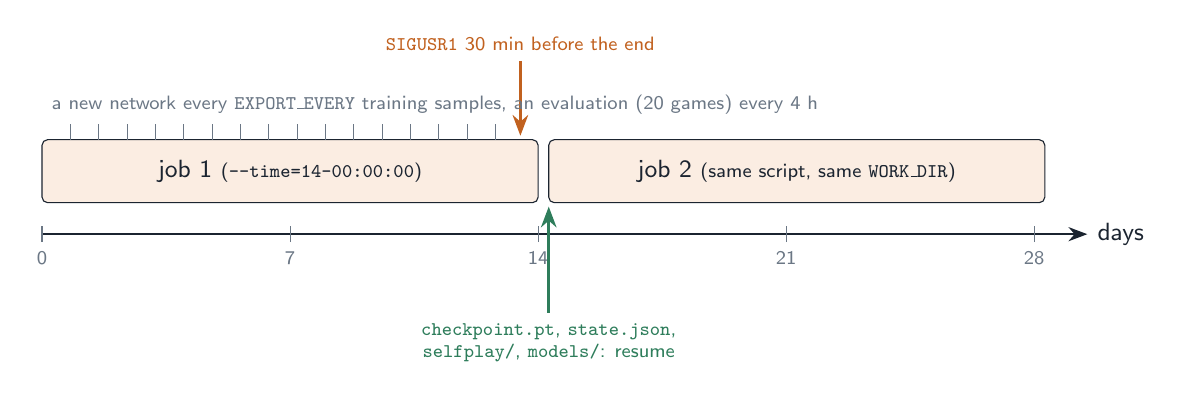
\begin{tikzpicture}[x=4.5mm,y=1mm]
  \draw[ar] (0,0) -- (29.5,0) node[plain,right]{days};
  \foreach \d in {0,7,14,21,28} { \draw[muted] (\d,-1) -- (\d,1); \node[tiny,below] at (\d,-1) {\d}; }
  \fill[soft2,draw=ink,rounded corners=2pt] (0,4) rectangle (14,12); \node[plain] at (7,8) {job 1 \scriptsize(\texttt{--time=14-00:00:00})};
  \fill[soft2,draw=ink,rounded corners=2pt] (14.3,4) rectangle (28.3,12); \node[plain] at (21.3,8) {job 2 \scriptsize(same script, same \texttt{WORK\_DIR})};
  \draw[accent2,line width=1pt,-{Stealth}] (13.5,22) node[tiny,above,text=accent2]{\texttt{SIGUSR1} 30 min before the end} -- (13.5,12.5);
  \draw[good,line width=1pt,-{Stealth}] (14.3,-10) node[tiny,below,text=good,align=center]{\texttt{checkpoint.pt}, \texttt{state.json},\\\texttt{selfplay/}, \texttt{models/}: resume} -- (14.3,3.5);
  \foreach \x in {0.8,1.6,...,13.2} \draw[muted] (\x,12) -- (\x,14);
  \node[tiny,anchor=west] at (0,16.5) {a new network every \texttt{EXPORT\_EVERY} training samples, an evaluation (20 games) every 4 h};
\end{tikzpicture}
\end{document}
